\documentclass[twoside]{book}

% Packages required by doxygen
\usepackage{fixltx2e}
\usepackage{calc}
\usepackage{doxygen}
\usepackage[export]{adjustbox} % also loads graphicx
\usepackage{graphicx}
\usepackage[utf8]{inputenc}
\usepackage{makeidx}
\usepackage{multicol}
\usepackage{multirow}
\PassOptionsToPackage{warn}{textcomp}
\usepackage{textcomp}
\usepackage[nointegrals]{wasysym}
\usepackage[table]{xcolor}

% Font selection
\usepackage[T1]{fontenc}
\usepackage[scaled=.90]{helvet}
\usepackage{courier}
\usepackage{amssymb}
\usepackage{sectsty}
\renewcommand{\familydefault}{\sfdefault}
\allsectionsfont{%
  \fontseries{bc}\selectfont%
  \color{darkgray}%
}
\renewcommand{\DoxyLabelFont}{%
  \fontseries{bc}\selectfont%
  \color{darkgray}%
}
\newcommand{\+}{\discretionary{\mbox{\scriptsize$\hookleftarrow$}}{}{}}

% Page & text layout
\usepackage{geometry}
\geometry{%
  a4paper,%
  top=2.5cm,%
  bottom=2.5cm,%
  left=2.5cm,%
  right=2.5cm%
}
\tolerance=750
\hfuzz=15pt
\hbadness=750
\setlength{\emergencystretch}{15pt}
\setlength{\parindent}{0cm}
\setlength{\parskip}{3ex plus 2ex minus 2ex}
\makeatletter
\renewcommand{\paragraph}{%
  \@startsection{paragraph}{4}{0ex}{-1.0ex}{1.0ex}{%
    \normalfont\normalsize\bfseries\SS@parafont%
  }%
}
\renewcommand{\subparagraph}{%
  \@startsection{subparagraph}{5}{0ex}{-1.0ex}{1.0ex}{%
    \normalfont\normalsize\bfseries\SS@subparafont%
  }%
}
\makeatother

% Headers & footers
\usepackage{fancyhdr}
\pagestyle{fancyplain}
\fancyhead[LE]{\fancyplain{}{\bfseries\thepage}}
\fancyhead[CE]{\fancyplain{}{}}
\fancyhead[RE]{\fancyplain{}{\bfseries\leftmark}}
\fancyhead[LO]{\fancyplain{}{\bfseries\rightmark}}
\fancyhead[CO]{\fancyplain{}{}}
\fancyhead[RO]{\fancyplain{}{\bfseries\thepage}}
\fancyfoot[LE]{\fancyplain{}{}}
\fancyfoot[CE]{\fancyplain{}{}}
\fancyfoot[RE]{\fancyplain{}{\bfseries\scriptsize Generated by Doxygen }}
\fancyfoot[LO]{\fancyplain{}{\bfseries\scriptsize Generated by Doxygen }}
\fancyfoot[CO]{\fancyplain{}{}}
\fancyfoot[RO]{\fancyplain{}{}}
\renewcommand{\footrulewidth}{0.4pt}
\renewcommand{\chaptermark}[1]{%
  \markboth{#1}{}%
}
\renewcommand{\sectionmark}[1]{%
  \markright{\thesection\ #1}%
}

% Indices & bibliography
\usepackage{natbib}
\usepackage[titles]{tocloft}
\setcounter{tocdepth}{3}
\setcounter{secnumdepth}{5}
\makeindex

% Hyperlinks (required, but should be loaded last)
\usepackage{ifpdf}
\ifpdf
  \usepackage[pdftex,pagebackref=true]{hyperref}
\else
  \usepackage[ps2pdf,pagebackref=true]{hyperref}
\fi
\hypersetup{%
  colorlinks=true,%
  linkcolor=blue,%
  citecolor=blue,%
  unicode%
}

% Custom commands
\newcommand{\clearemptydoublepage}{%
  \newpage{\pagestyle{empty}\cleardoublepage}%
}

\usepackage{caption}
\captionsetup{labelsep=space,justification=centering,font={bf},singlelinecheck=off,skip=4pt,position=top}

%===== C O N T E N T S =====

\begin{document}

% Titlepage & ToC
\hypersetup{pageanchor=false,
             bookmarksnumbered=true,
             pdfencoding=unicode
            }
\pagenumbering{roman}
\begin{titlepage}
\vspace*{7cm}
\begin{center}%
{\Large My Project }\\
\vspace*{1cm}
{\large Generated by Doxygen 1.8.11}\\
\end{center}
\end{titlepage}
\clearemptydoublepage
\tableofcontents
\clearemptydoublepage
\pagenumbering{arabic}
\hypersetup{pageanchor=true}

%--- Begin generated contents ---
\chapter{Hierarchical Index}
\section{Class Hierarchy}
This inheritance list is sorted roughly, but not completely, alphabetically\+:\begin{DoxyCompactList}
\item \contentsline{section}{Fruit}{\pageref{classFruit}}{}
\begin{DoxyCompactList}
\item \contentsline{section}{Apple}{\pageref{classApple}}{}
\item \contentsline{section}{Grape}{\pageref{classGrape}}{}
\item \contentsline{section}{Orange}{\pageref{classOrange}}{}
\end{DoxyCompactList}
\item \contentsline{section}{List}{\pageref{classList}}{}
\item \contentsline{section}{List\+:\+:Node}{\pageref{structList_1_1Node}}{}
\end{DoxyCompactList}

\chapter{Class Index}
\section{Class List}
Here are the classes, structs, unions and interfaces with brief descriptions\+:\begin{DoxyCompactList}
\item\contentsline{section}{\hyperlink{structnode}{node} }{\pageref{structnode}}{}
\item\contentsline{section}{\hyperlink{structnode1}{node1} }{\pageref{structnode1}}{}
\item\contentsline{section}{\hyperlink{structnode__info}{node\+\_\+info} }{\pageref{structnode__info}}{}
\end{DoxyCompactList}

\chapter{File Index}
\section{File List}
Here is a list of all files with brief descriptions\+:\begin{DoxyCompactList}
\item\contentsline{section}{\hyperlink{Lab1_8c}{Lab1.\+c} }{\pageref{Lab1_8c}}{}
\end{DoxyCompactList}

\chapter{Class Documentation}
\hypertarget{classBikeRecord}{}\section{Bike\+Record Class Reference}
\label{classBikeRecord}\index{Bike\+Record@{Bike\+Record}}


Inheritance diagram for Bike\+Record\+:\nopagebreak
\begin{figure}[H]
\begin{center}
\leavevmode
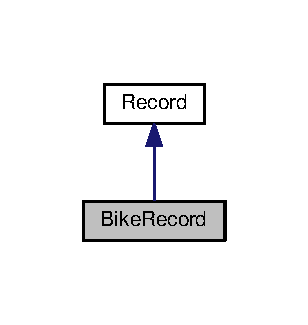
\includegraphics[width=148pt]{classBikeRecord__inherit__graph}
\end{center}
\end{figure}


Collaboration diagram for Bike\+Record\+:\nopagebreak
\begin{figure}[H]
\begin{center}
\leavevmode
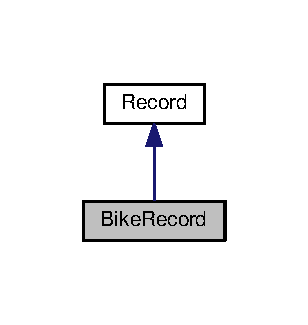
\includegraphics[width=148pt]{classBikeRecord__coll__graph}
\end{center}
\end{figure}
\subsection*{Public Member Functions}
\begin{DoxyCompactItemize}
\item 
\hyperlink{classBikeRecord_aeb895d757c28796857eac6f246098e45}{Bike\+Record} (string bike\+Name, int ID)
\item 
void \hyperlink{classBikeRecord_a84eee4b442a8a82a131f595915a3f4ce}{print} () override
\item 
\hyperlink{classRecord}{Record} $\ast$ \hyperlink{classBikeRecord_a306fa32f6acb1c27a2e2d2f353cff9c8}{clone} () override
\end{DoxyCompactItemize}
\subsection*{Private Attributes}
\begin{DoxyCompactItemize}
\item 
string \hyperlink{classBikeRecord_a5d1749281f51f57f778d11873beb8fdd}{m\+\_\+bike\+Name}
\item 
int \hyperlink{classBikeRecord_a1539b267352308b9ac0a97c54291aafd}{m\+\_\+\+ID}
\end{DoxyCompactItemize}


\subsection{Detailed Description}
\hyperlink{classBikeRecord}{Bike\+Record} is the Concrete Prototype 

\subsection{Constructor \& Destructor Documentation}
\index{Bike\+Record@{Bike\+Record}!Bike\+Record@{Bike\+Record}}
\index{Bike\+Record@{Bike\+Record}!Bike\+Record@{Bike\+Record}}
\subsubsection[{\texorpdfstring{Bike\+Record(string bike\+Name, int I\+D)}{BikeRecord(string bikeName, int ID)}}]{\setlength{\rightskip}{0pt plus 5cm}Bike\+Record\+::\+Bike\+Record (
\begin{DoxyParamCaption}
\item[{string}]{bike\+Name, }
\item[{int}]{ID}
\end{DoxyParamCaption}
)\hspace{0.3cm}{\ttfamily [inline]}}\hypertarget{classBikeRecord_aeb895d757c28796857eac6f246098e45}{}\label{classBikeRecord_aeb895d757c28796857eac6f246098e45}

\begin{DoxyCode}
50                                         : \hyperlink{classBikeRecord_a5d1749281f51f57f778d11873beb8fdd}{m\_bikeName}(bikeName), \hyperlink{classBikeRecord_a1539b267352308b9ac0a97c54291aafd}{m\_ID}(ID)
51     \{
52     \}
\end{DoxyCode}


\subsection{Member Function Documentation}
\index{Bike\+Record@{Bike\+Record}!clone@{clone}}
\index{clone@{clone}!Bike\+Record@{Bike\+Record}}
\subsubsection[{\texorpdfstring{clone() override}{clone() override}}]{\setlength{\rightskip}{0pt plus 5cm}{\bf Record}$\ast$ Bike\+Record\+::clone (
\begin{DoxyParamCaption}
{}
\end{DoxyParamCaption}
)\hspace{0.3cm}{\ttfamily [inline]}, {\ttfamily [override]}, {\ttfamily [virtual]}}\hypertarget{classBikeRecord_a306fa32f6acb1c27a2e2d2f353cff9c8}{}\label{classBikeRecord_a306fa32f6acb1c27a2e2d2f353cff9c8}


Implements \hyperlink{classRecord_a78dec14d71a48508de135ee06fe48373}{Record}.


\begin{DoxyCode}
62     \{
63         \textcolor{keywordflow}{return} \textcolor{keyword}{new} \hyperlink{classBikeRecord_aeb895d757c28796857eac6f246098e45}{BikeRecord}(*\textcolor{keyword}{this});
64     \}
\end{DoxyCode}
\index{Bike\+Record@{Bike\+Record}!print@{print}}
\index{print@{print}!Bike\+Record@{Bike\+Record}}
\subsubsection[{\texorpdfstring{print() override}{print() override}}]{\setlength{\rightskip}{0pt plus 5cm}void Bike\+Record\+::print (
\begin{DoxyParamCaption}
{}
\end{DoxyParamCaption}
)\hspace{0.3cm}{\ttfamily [inline]}, {\ttfamily [override]}, {\ttfamily [virtual]}}\hypertarget{classBikeRecord_a84eee4b442a8a82a131f595915a3f4ce}{}\label{classBikeRecord_a84eee4b442a8a82a131f595915a3f4ce}


Implements \hyperlink{classRecord_ad218b1bea934fb19a23a35b0b987e033}{Record}.


\begin{DoxyCode}
55     \{
56         cout << \textcolor{stringliteral}{"Bike Record"} << endl
57              << \textcolor{stringliteral}{"Name  : "} << \hyperlink{classBikeRecord_a5d1749281f51f57f778d11873beb8fdd}{m\_bikeName} << endl
58              << \textcolor{stringliteral}{"Number: "} << \hyperlink{classBikeRecord_a1539b267352308b9ac0a97c54291aafd}{m\_ID} << endl << endl;
59     \}
\end{DoxyCode}


\subsection{Member Data Documentation}
\index{Bike\+Record@{Bike\+Record}!m\+\_\+bike\+Name@{m\+\_\+bike\+Name}}
\index{m\+\_\+bike\+Name@{m\+\_\+bike\+Name}!Bike\+Record@{Bike\+Record}}
\subsubsection[{\texorpdfstring{m\+\_\+bike\+Name}{m_bikeName}}]{\setlength{\rightskip}{0pt plus 5cm}string Bike\+Record\+::m\+\_\+bike\+Name\hspace{0.3cm}{\ttfamily [private]}}\hypertarget{classBikeRecord_a5d1749281f51f57f778d11873beb8fdd}{}\label{classBikeRecord_a5d1749281f51f57f778d11873beb8fdd}
\index{Bike\+Record@{Bike\+Record}!m\+\_\+\+ID@{m\+\_\+\+ID}}
\index{m\+\_\+\+ID@{m\+\_\+\+ID}!Bike\+Record@{Bike\+Record}}
\subsubsection[{\texorpdfstring{m\+\_\+\+ID}{m_ID}}]{\setlength{\rightskip}{0pt plus 5cm}int Bike\+Record\+::m\+\_\+\+ID\hspace{0.3cm}{\ttfamily [private]}}\hypertarget{classBikeRecord_a1539b267352308b9ac0a97c54291aafd}{}\label{classBikeRecord_a1539b267352308b9ac0a97c54291aafd}


The documentation for this class was generated from the following file\+:\begin{DoxyCompactItemize}
\item 
\hyperlink{Prototype_8cpp}{Prototype.\+cpp}\end{DoxyCompactItemize}

\hypertarget{classCarRecord}{}\section{Car\+Record Class Reference}
\label{classCarRecord}\index{Car\+Record@{Car\+Record}}


Inheritance diagram for Car\+Record\+:\nopagebreak
\begin{figure}[H]
\begin{center}
\leavevmode
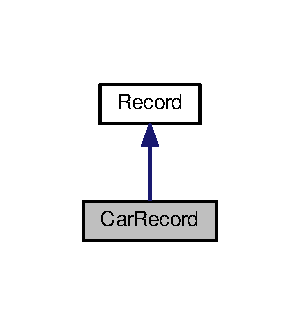
\includegraphics[width=144pt]{classCarRecord__inherit__graph}
\end{center}
\end{figure}


Collaboration diagram for Car\+Record\+:\nopagebreak
\begin{figure}[H]
\begin{center}
\leavevmode
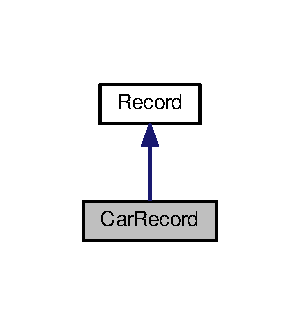
\includegraphics[width=144pt]{classCarRecord__coll__graph}
\end{center}
\end{figure}
\subsection*{Public Member Functions}
\begin{DoxyCompactItemize}
\item 
\hyperlink{classCarRecord_ab1ff8a8eb47b4792718a2eff6012656e}{Car\+Record} (string car\+Name, int ID)
\item 
void \hyperlink{classCarRecord_a84789b5f6a61048c481d115c7058d664}{print} () override
\item 
\hyperlink{classRecord}{Record} $\ast$ \hyperlink{classCarRecord_a190ab69e95107c689455fd85099f3630}{clone} () override
\end{DoxyCompactItemize}
\subsection*{Private Attributes}
\begin{DoxyCompactItemize}
\item 
string \hyperlink{classCarRecord_a11d736579cd5caeb73076ec2b5ca59ba}{m\+\_\+car\+Name}
\item 
int \hyperlink{classCarRecord_a2ec8ef22ca91cb79481b189cfa9dce7c}{m\+\_\+\+ID}
\end{DoxyCompactItemize}


\subsection{Detailed Description}
\hyperlink{classCarRecord}{Car\+Record} is a Concrete Prototype 

\subsection{Constructor \& Destructor Documentation}
\index{Car\+Record@{Car\+Record}!Car\+Record@{Car\+Record}}
\index{Car\+Record@{Car\+Record}!Car\+Record@{Car\+Record}}
\subsubsection[{\texorpdfstring{Car\+Record(string car\+Name, int I\+D)}{CarRecord(string carName, int ID)}}]{\setlength{\rightskip}{0pt plus 5cm}Car\+Record\+::\+Car\+Record (
\begin{DoxyParamCaption}
\item[{string}]{car\+Name, }
\item[{int}]{ID}
\end{DoxyParamCaption}
)\hspace{0.3cm}{\ttfamily [inline]}}\hypertarget{classCarRecord_ab1ff8a8eb47b4792718a2eff6012656e}{}\label{classCarRecord_ab1ff8a8eb47b4792718a2eff6012656e}

\begin{DoxyCode}
25                                       : \hyperlink{classCarRecord_a11d736579cd5caeb73076ec2b5ca59ba}{m\_carName}(carName), \hyperlink{classCarRecord_a2ec8ef22ca91cb79481b189cfa9dce7c}{m\_ID}(ID)
26     \{
27     \}
\end{DoxyCode}


\subsection{Member Function Documentation}
\index{Car\+Record@{Car\+Record}!clone@{clone}}
\index{clone@{clone}!Car\+Record@{Car\+Record}}
\subsubsection[{\texorpdfstring{clone() override}{clone() override}}]{\setlength{\rightskip}{0pt plus 5cm}{\bf Record}$\ast$ Car\+Record\+::clone (
\begin{DoxyParamCaption}
{}
\end{DoxyParamCaption}
)\hspace{0.3cm}{\ttfamily [inline]}, {\ttfamily [override]}, {\ttfamily [virtual]}}\hypertarget{classCarRecord_a190ab69e95107c689455fd85099f3630}{}\label{classCarRecord_a190ab69e95107c689455fd85099f3630}


Implements \hyperlink{classRecord_a78dec14d71a48508de135ee06fe48373}{Record}.


\begin{DoxyCode}
37     \{
38         \textcolor{keywordflow}{return} \textcolor{keyword}{new} \hyperlink{classCarRecord_ab1ff8a8eb47b4792718a2eff6012656e}{CarRecord}(*\textcolor{keyword}{this});
39     \}
\end{DoxyCode}
\index{Car\+Record@{Car\+Record}!print@{print}}
\index{print@{print}!Car\+Record@{Car\+Record}}
\subsubsection[{\texorpdfstring{print() override}{print() override}}]{\setlength{\rightskip}{0pt plus 5cm}void Car\+Record\+::print (
\begin{DoxyParamCaption}
{}
\end{DoxyParamCaption}
)\hspace{0.3cm}{\ttfamily [inline]}, {\ttfamily [override]}, {\ttfamily [virtual]}}\hypertarget{classCarRecord_a84789b5f6a61048c481d115c7058d664}{}\label{classCarRecord_a84789b5f6a61048c481d115c7058d664}


Implements \hyperlink{classRecord_ad218b1bea934fb19a23a35b0b987e033}{Record}.


\begin{DoxyCode}
30     \{
31         cout << \textcolor{stringliteral}{"Car Record"} << endl
32              << \textcolor{stringliteral}{"Name  : "}   << \hyperlink{classCarRecord_a11d736579cd5caeb73076ec2b5ca59ba}{m\_carName} << endl
33              << \textcolor{stringliteral}{"Number: "}   << \hyperlink{classCarRecord_a2ec8ef22ca91cb79481b189cfa9dce7c}{m\_ID} << endl << endl;
34     \}
\end{DoxyCode}


\subsection{Member Data Documentation}
\index{Car\+Record@{Car\+Record}!m\+\_\+car\+Name@{m\+\_\+car\+Name}}
\index{m\+\_\+car\+Name@{m\+\_\+car\+Name}!Car\+Record@{Car\+Record}}
\subsubsection[{\texorpdfstring{m\+\_\+car\+Name}{m_carName}}]{\setlength{\rightskip}{0pt plus 5cm}string Car\+Record\+::m\+\_\+car\+Name\hspace{0.3cm}{\ttfamily [private]}}\hypertarget{classCarRecord_a11d736579cd5caeb73076ec2b5ca59ba}{}\label{classCarRecord_a11d736579cd5caeb73076ec2b5ca59ba}
\index{Car\+Record@{Car\+Record}!m\+\_\+\+ID@{m\+\_\+\+ID}}
\index{m\+\_\+\+ID@{m\+\_\+\+ID}!Car\+Record@{Car\+Record}}
\subsubsection[{\texorpdfstring{m\+\_\+\+ID}{m_ID}}]{\setlength{\rightskip}{0pt plus 5cm}int Car\+Record\+::m\+\_\+\+ID\hspace{0.3cm}{\ttfamily [private]}}\hypertarget{classCarRecord_a2ec8ef22ca91cb79481b189cfa9dce7c}{}\label{classCarRecord_a2ec8ef22ca91cb79481b189cfa9dce7c}


The documentation for this class was generated from the following file\+:\begin{DoxyCompactItemize}
\item 
\hyperlink{Prototype_8cpp}{Prototype.\+cpp}\end{DoxyCompactItemize}

\hypertarget{classPersonRecord}{}\section{Person\+Record Class Reference}
\label{classPersonRecord}\index{Person\+Record@{Person\+Record}}


Inheritance diagram for Person\+Record\+:\nopagebreak
\begin{figure}[H]
\begin{center}
\leavevmode
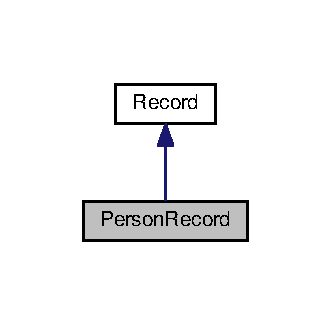
\includegraphics[width=159pt]{classPersonRecord__inherit__graph}
\end{center}
\end{figure}


Collaboration diagram for Person\+Record\+:\nopagebreak
\begin{figure}[H]
\begin{center}
\leavevmode
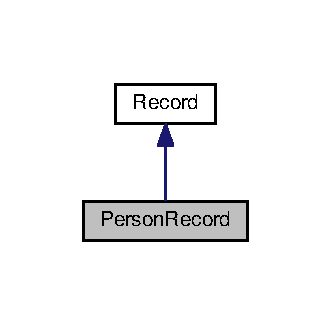
\includegraphics[width=159pt]{classPersonRecord__coll__graph}
\end{center}
\end{figure}
\subsection*{Public Member Functions}
\begin{DoxyCompactItemize}
\item 
\hyperlink{classPersonRecord_a124548640e4d2075933e176f86d09e04}{Person\+Record} (string person\+Name, int age)
\item 
void \hyperlink{classPersonRecord_a5e4de1bb08b2d52adf778cda7aeb71ee}{print} () override
\item 
\hyperlink{classRecord}{Record} $\ast$ \hyperlink{classPersonRecord_a52c028d43ada61bb5b96c162569fbed3}{clone} () override
\end{DoxyCompactItemize}
\subsection*{Private Attributes}
\begin{DoxyCompactItemize}
\item 
string \hyperlink{classPersonRecord_af9c4e5c960723d9da2a1fd48c54d2404}{m\+\_\+person\+Name}
\item 
int \hyperlink{classPersonRecord_a5c3c3ed331d3b814e67922d0f4c0a13f}{m\+\_\+age}
\end{DoxyCompactItemize}


\subsection{Detailed Description}
\hyperlink{classPersonRecord}{Person\+Record} is the Concrete Prototype 

\subsection{Constructor \& Destructor Documentation}
\index{Person\+Record@{Person\+Record}!Person\+Record@{Person\+Record}}
\index{Person\+Record@{Person\+Record}!Person\+Record@{Person\+Record}}
\subsubsection[{\texorpdfstring{Person\+Record(string person\+Name, int age)}{PersonRecord(string personName, int age)}}]{\setlength{\rightskip}{0pt plus 5cm}Person\+Record\+::\+Person\+Record (
\begin{DoxyParamCaption}
\item[{string}]{person\+Name, }
\item[{int}]{age}
\end{DoxyParamCaption}
)\hspace{0.3cm}{\ttfamily [inline]}}\hypertarget{classPersonRecord_a124548640e4d2075933e176f86d09e04}{}\label{classPersonRecord_a124548640e4d2075933e176f86d09e04}

\begin{DoxyCode}
75                                              : \hyperlink{classPersonRecord_af9c4e5c960723d9da2a1fd48c54d2404}{m\_personName}(personName), 
      \hyperlink{classPersonRecord_a5c3c3ed331d3b814e67922d0f4c0a13f}{m\_age}(age)
76     \{
77     \}
\end{DoxyCode}


\subsection{Member Function Documentation}
\index{Person\+Record@{Person\+Record}!clone@{clone}}
\index{clone@{clone}!Person\+Record@{Person\+Record}}
\subsubsection[{\texorpdfstring{clone() override}{clone() override}}]{\setlength{\rightskip}{0pt plus 5cm}{\bf Record}$\ast$ Person\+Record\+::clone (
\begin{DoxyParamCaption}
{}
\end{DoxyParamCaption}
)\hspace{0.3cm}{\ttfamily [inline]}, {\ttfamily [override]}, {\ttfamily [virtual]}}\hypertarget{classPersonRecord_a52c028d43ada61bb5b96c162569fbed3}{}\label{classPersonRecord_a52c028d43ada61bb5b96c162569fbed3}


Implements \hyperlink{classRecord_a78dec14d71a48508de135ee06fe48373}{Record}.


\begin{DoxyCode}
87     \{
88         \textcolor{keywordflow}{return} \textcolor{keyword}{new} \hyperlink{classPersonRecord_a124548640e4d2075933e176f86d09e04}{PersonRecord}(*\textcolor{keyword}{this});
89     \}
\end{DoxyCode}
\index{Person\+Record@{Person\+Record}!print@{print}}
\index{print@{print}!Person\+Record@{Person\+Record}}
\subsubsection[{\texorpdfstring{print() override}{print() override}}]{\setlength{\rightskip}{0pt plus 5cm}void Person\+Record\+::print (
\begin{DoxyParamCaption}
{}
\end{DoxyParamCaption}
)\hspace{0.3cm}{\ttfamily [inline]}, {\ttfamily [override]}, {\ttfamily [virtual]}}\hypertarget{classPersonRecord_a5e4de1bb08b2d52adf778cda7aeb71ee}{}\label{classPersonRecord_a5e4de1bb08b2d52adf778cda7aeb71ee}


Implements \hyperlink{classRecord_ad218b1bea934fb19a23a35b0b987e033}{Record}.


\begin{DoxyCode}
80     \{
81         cout << \textcolor{stringliteral}{"Person Record"} << endl
82             << \textcolor{stringliteral}{"Name : "} << \hyperlink{classPersonRecord_af9c4e5c960723d9da2a1fd48c54d2404}{m\_personName} << endl
83             << \textcolor{stringliteral}{"Age  : "} << \hyperlink{classPersonRecord_a5c3c3ed331d3b814e67922d0f4c0a13f}{m\_age} << endl << endl;
84     \}
\end{DoxyCode}


\subsection{Member Data Documentation}
\index{Person\+Record@{Person\+Record}!m\+\_\+age@{m\+\_\+age}}
\index{m\+\_\+age@{m\+\_\+age}!Person\+Record@{Person\+Record}}
\subsubsection[{\texorpdfstring{m\+\_\+age}{m_age}}]{\setlength{\rightskip}{0pt plus 5cm}int Person\+Record\+::m\+\_\+age\hspace{0.3cm}{\ttfamily [private]}}\hypertarget{classPersonRecord_a5c3c3ed331d3b814e67922d0f4c0a13f}{}\label{classPersonRecord_a5c3c3ed331d3b814e67922d0f4c0a13f}
\index{Person\+Record@{Person\+Record}!m\+\_\+person\+Name@{m\+\_\+person\+Name}}
\index{m\+\_\+person\+Name@{m\+\_\+person\+Name}!Person\+Record@{Person\+Record}}
\subsubsection[{\texorpdfstring{m\+\_\+person\+Name}{m_personName}}]{\setlength{\rightskip}{0pt plus 5cm}string Person\+Record\+::m\+\_\+person\+Name\hspace{0.3cm}{\ttfamily [private]}}\hypertarget{classPersonRecord_af9c4e5c960723d9da2a1fd48c54d2404}{}\label{classPersonRecord_af9c4e5c960723d9da2a1fd48c54d2404}


The documentation for this class was generated from the following file\+:\begin{DoxyCompactItemize}
\item 
\hyperlink{Prototype_8cpp}{Prototype.\+cpp}\end{DoxyCompactItemize}

\hypertarget{classRecord}{}\section{Record Class Reference}
\label{classRecord}\index{Record@{Record}}


Inheritance diagram for Record\+:\nopagebreak
\begin{figure}[H]
\begin{center}
\leavevmode
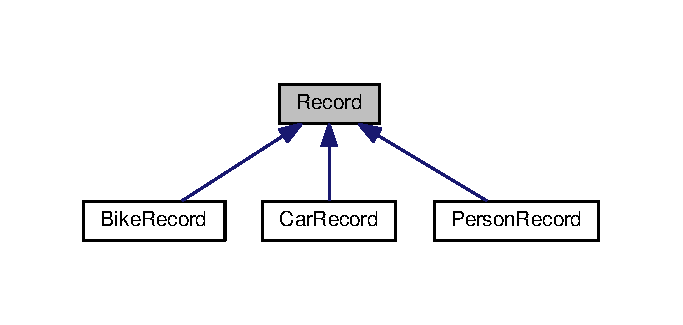
\includegraphics[width=328pt]{classRecord__inherit__graph}
\end{center}
\end{figure}
\subsection*{Public Member Functions}
\begin{DoxyCompactItemize}
\item 
virtual \hyperlink{classRecord_a6b457aa68799196febbe2821c82b042e}{$\sim$\+Record} ()
\item 
virtual void \hyperlink{classRecord_ad218b1bea934fb19a23a35b0b987e033}{print} ()=0
\item 
virtual \hyperlink{classRecord}{Record} $\ast$ \hyperlink{classRecord_a78dec14d71a48508de135ee06fe48373}{clone} ()=0
\end{DoxyCompactItemize}


\subsection{Detailed Description}
\hyperlink{classRecord}{Record} is the base Prototype 

\subsection{Constructor \& Destructor Documentation}
\index{Record@{Record}!````~Record@{$\sim$\+Record}}
\index{````~Record@{$\sim$\+Record}!Record@{Record}}
\subsubsection[{\texorpdfstring{$\sim$\+Record()}{~Record()}}]{\setlength{\rightskip}{0pt plus 5cm}virtual Record\+::$\sim$\+Record (
\begin{DoxyParamCaption}
{}
\end{DoxyParamCaption}
)\hspace{0.3cm}{\ttfamily [inline]}, {\ttfamily [virtual]}}\hypertarget{classRecord_a6b457aa68799196febbe2821c82b042e}{}\label{classRecord_a6b457aa68799196febbe2821c82b042e}

\begin{DoxyCode}
12 \{\}
\end{DoxyCode}


\subsection{Member Function Documentation}
\index{Record@{Record}!clone@{clone}}
\index{clone@{clone}!Record@{Record}}
\subsubsection[{\texorpdfstring{clone()=0}{clone()=0}}]{\setlength{\rightskip}{0pt plus 5cm}virtual {\bf Record}$\ast$ Record\+::clone (
\begin{DoxyParamCaption}
{}
\end{DoxyParamCaption}
)\hspace{0.3cm}{\ttfamily [pure virtual]}}\hypertarget{classRecord_a78dec14d71a48508de135ee06fe48373}{}\label{classRecord_a78dec14d71a48508de135ee06fe48373}


Implemented in \hyperlink{classPersonRecord_a52c028d43ada61bb5b96c162569fbed3}{Person\+Record}, \hyperlink{classBikeRecord_a306fa32f6acb1c27a2e2d2f353cff9c8}{Bike\+Record}, and \hyperlink{classCarRecord_a190ab69e95107c689455fd85099f3630}{Car\+Record}.

\index{Record@{Record}!print@{print}}
\index{print@{print}!Record@{Record}}
\subsubsection[{\texorpdfstring{print()=0}{print()=0}}]{\setlength{\rightskip}{0pt plus 5cm}virtual void Record\+::print (
\begin{DoxyParamCaption}
{}
\end{DoxyParamCaption}
)\hspace{0.3cm}{\ttfamily [pure virtual]}}\hypertarget{classRecord_ad218b1bea934fb19a23a35b0b987e033}{}\label{classRecord_ad218b1bea934fb19a23a35b0b987e033}


Implemented in \hyperlink{classPersonRecord_a5e4de1bb08b2d52adf778cda7aeb71ee}{Person\+Record}, \hyperlink{classBikeRecord_a84eee4b442a8a82a131f595915a3f4ce}{Bike\+Record}, and \hyperlink{classCarRecord_a84789b5f6a61048c481d115c7058d664}{Car\+Record}.



The documentation for this class was generated from the following file\+:\begin{DoxyCompactItemize}
\item 
\hyperlink{Prototype_8cpp}{Prototype.\+cpp}\end{DoxyCompactItemize}

\hypertarget{classRecordFactory}{}\section{Record\+Factory Class Reference}
\label{classRecordFactory}\index{Record\+Factory@{Record\+Factory}}
\subsection*{Public Member Functions}
\begin{DoxyCompactItemize}
\item 
\hyperlink{classRecordFactory_a2c744c160d1f25c5abee97372979201c}{Record\+Factory} ()
\item 
\hyperlink{classRecord}{Record} $\ast$ \hyperlink{classRecordFactory_a0606dd9c40bc58a23f995bf39b4e5444}{create\+Record} (\hyperlink{Prototype_8cpp_ad7dc06ed9ae2cf0a910eed652dca9a44}{Record\+Type} record\+Type)
\end{DoxyCompactItemize}
\subsection*{Private Attributes}
\begin{DoxyCompactItemize}
\item 
unordered\+\_\+map$<$ \hyperlink{Prototype_8cpp_ad7dc06ed9ae2cf0a910eed652dca9a44}{Record\+Type}, \hyperlink{classRecord}{Record} $\ast$, hash$<$ int $>$ $>$ \hyperlink{classRecordFactory_a5a1de3c7661d204f37bfc7f077e873d0}{m\+\_\+records}
\end{DoxyCompactItemize}


\subsection{Detailed Description}
\hyperlink{classRecordFactory}{Record\+Factory} is the client 

\subsection{Constructor \& Destructor Documentation}
\index{Record\+Factory@{Record\+Factory}!Record\+Factory@{Record\+Factory}}
\index{Record\+Factory@{Record\+Factory}!Record\+Factory@{Record\+Factory}}
\subsubsection[{\texorpdfstring{Record\+Factory()}{RecordFactory()}}]{\setlength{\rightskip}{0pt plus 5cm}Record\+Factory\+::\+Record\+Factory (
\begin{DoxyParamCaption}
{}
\end{DoxyParamCaption}
)\hspace{0.3cm}{\ttfamily [inline]}}\hypertarget{classRecordFactory_a2c744c160d1f25c5abee97372979201c}{}\label{classRecordFactory_a2c744c160d1f25c5abee97372979201c}

\begin{DoxyCode}
108     \{
109         \hyperlink{classRecordFactory_a5a1de3c7661d204f37bfc7f077e873d0}{m\_records}[\hyperlink{Prototype_8cpp_ad7dc06ed9ae2cf0a910eed652dca9a44a5fc54ebcb1dd4bf1e1b93cbc77b57b40}{CAR}]    = \textcolor{keyword}{new} \hyperlink{classCarRecord}{CarRecord}(\textcolor{stringliteral}{"Ferrari"}, 5050);
110         \hyperlink{classRecordFactory_a5a1de3c7661d204f37bfc7f077e873d0}{m\_records}[\hyperlink{Prototype_8cpp_ad7dc06ed9ae2cf0a910eed652dca9a44a5728381009aee1446c2b7d19c35c9c15}{BIKE}]   = \textcolor{keyword}{new} \hyperlink{classBikeRecord}{BikeRecord}(\textcolor{stringliteral}{"Yamaha"}, 2525);
111         \hyperlink{classRecordFactory_a5a1de3c7661d204f37bfc7f077e873d0}{m\_records}[\hyperlink{Prototype_8cpp_ad7dc06ed9ae2cf0a910eed652dca9a44ac9878c552c3ddcde707fff8aefa250ae}{PERSON}] = \textcolor{keyword}{new} \hyperlink{classPersonRecord}{PersonRecord}(\textcolor{stringliteral}{"Tom"}, 25);
112     \}
\end{DoxyCode}


\subsection{Member Function Documentation}
\index{Record\+Factory@{Record\+Factory}!create\+Record@{create\+Record}}
\index{create\+Record@{create\+Record}!Record\+Factory@{Record\+Factory}}
\subsubsection[{\texorpdfstring{create\+Record(\+Record\+Type record\+Type)}{createRecord(RecordType recordType)}}]{\setlength{\rightskip}{0pt plus 5cm}{\bf Record}$\ast$ Record\+Factory\+::create\+Record (
\begin{DoxyParamCaption}
\item[{{\bf Record\+Type}}]{record\+Type}
\end{DoxyParamCaption}
)\hspace{0.3cm}{\ttfamily [inline]}}\hypertarget{classRecordFactory_a0606dd9c40bc58a23f995bf39b4e5444}{}\label{classRecordFactory_a0606dd9c40bc58a23f995bf39b4e5444}

\begin{DoxyCode}
115     \{
116         \textcolor{keywordflow}{return} \hyperlink{classRecordFactory_a5a1de3c7661d204f37bfc7f077e873d0}{m\_records}[recordType]->clone();
117     \}
\end{DoxyCode}


Here is the call graph for this function\+:
\nopagebreak
\begin{figure}[H]
\begin{center}
\leavevmode
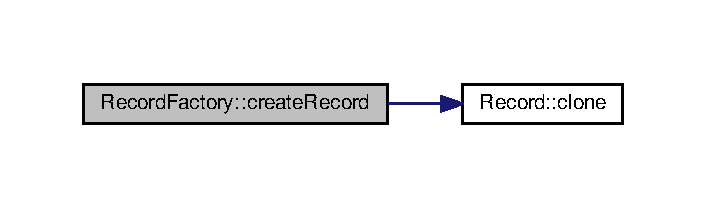
\includegraphics[width=339pt]{classRecordFactory_a0606dd9c40bc58a23f995bf39b4e5444_cgraph}
\end{center}
\end{figure}




\subsection{Member Data Documentation}
\index{Record\+Factory@{Record\+Factory}!m\+\_\+records@{m\+\_\+records}}
\index{m\+\_\+records@{m\+\_\+records}!Record\+Factory@{Record\+Factory}}
\subsubsection[{\texorpdfstring{m\+\_\+records}{m_records}}]{\setlength{\rightskip}{0pt plus 5cm}unordered\+\_\+map$<${\bf Record\+Type}, {\bf Record}$\ast$, hash$<$int$>$ $>$ Record\+Factory\+::m\+\_\+records\hspace{0.3cm}{\ttfamily [private]}}\hypertarget{classRecordFactory_a5a1de3c7661d204f37bfc7f077e873d0}{}\label{classRecordFactory_a5a1de3c7661d204f37bfc7f077e873d0}


The documentation for this class was generated from the following file\+:\begin{DoxyCompactItemize}
\item 
\hyperlink{Prototype_8cpp}{Prototype.\+cpp}\end{DoxyCompactItemize}

\chapter{File Documentation}
\hypertarget{Prototype_8cpp}{}\section{Prototype.\+cpp File Reference}
\label{Prototype_8cpp}\index{Prototype.\+cpp@{Prototype.\+cpp}}
{\ttfamily \#include $<$iostream$>$}\\*
{\ttfamily \#include $<$unordered\+\_\+map$>$}\\*
{\ttfamily \#include $<$string$>$}\\*
{\ttfamily \#include $<$memory$>$}\\*
Include dependency graph for Prototype.\+cpp\+:\nopagebreak
\begin{figure}[H]
\begin{center}
\leavevmode
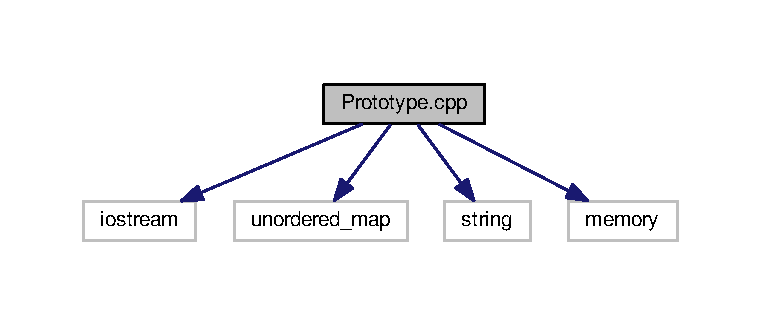
\includegraphics[width=350pt]{Prototype_8cpp__incl}
\end{center}
\end{figure}
\subsection*{Classes}
\begin{DoxyCompactItemize}
\item 
class \hyperlink{classRecord}{Record}
\item 
class \hyperlink{classCarRecord}{Car\+Record}
\item 
class \hyperlink{classBikeRecord}{Bike\+Record}
\item 
class \hyperlink{classPersonRecord}{Person\+Record}
\item 
class \hyperlink{classRecordFactory}{Record\+Factory}
\end{DoxyCompactItemize}
\subsection*{Enumerations}
\begin{DoxyCompactItemize}
\item 
enum \hyperlink{Prototype_8cpp_ad7dc06ed9ae2cf0a910eed652dca9a44}{Record\+Type} \{ \hyperlink{Prototype_8cpp_ad7dc06ed9ae2cf0a910eed652dca9a44a5fc54ebcb1dd4bf1e1b93cbc77b57b40}{C\+AR}, 
\hyperlink{Prototype_8cpp_ad7dc06ed9ae2cf0a910eed652dca9a44a5728381009aee1446c2b7d19c35c9c15}{B\+I\+KE}, 
\hyperlink{Prototype_8cpp_ad7dc06ed9ae2cf0a910eed652dca9a44ac9878c552c3ddcde707fff8aefa250ae}{P\+E\+R\+S\+ON}
 \}
\end{DoxyCompactItemize}
\subsection*{Functions}
\begin{DoxyCompactItemize}
\item 
int \hyperlink{Prototype_8cpp_ae66f6b31b5ad750f1fe042a706a4e3d4}{main} ()
\end{DoxyCompactItemize}


\subsection{Enumeration Type Documentation}
\index{Prototype.\+cpp@{Prototype.\+cpp}!Record\+Type@{Record\+Type}}
\index{Record\+Type@{Record\+Type}!Prototype.\+cpp@{Prototype.\+cpp}}
\subsubsection[{\texorpdfstring{Record\+Type}{RecordType}}]{\setlength{\rightskip}{0pt plus 5cm}enum {\bf Record\+Type}}\hypertarget{Prototype_8cpp_ad7dc06ed9ae2cf0a910eed652dca9a44}{}\label{Prototype_8cpp_ad7dc06ed9ae2cf0a910eed652dca9a44}
Opaque record type, avoids exposing concrete implementations \begin{Desc}
\item[Enumerator]\par
\begin{description}
\index{C\+AR@{C\+AR}!Prototype.\+cpp@{Prototype.\+cpp}}\index{Prototype.\+cpp@{Prototype.\+cpp}!C\+AR@{C\+AR}}\item[{\em 
C\+AR\hypertarget{Prototype_8cpp_ad7dc06ed9ae2cf0a910eed652dca9a44a5fc54ebcb1dd4bf1e1b93cbc77b57b40}{}\label{Prototype_8cpp_ad7dc06ed9ae2cf0a910eed652dca9a44a5fc54ebcb1dd4bf1e1b93cbc77b57b40}
}]\index{B\+I\+KE@{B\+I\+KE}!Prototype.\+cpp@{Prototype.\+cpp}}\index{Prototype.\+cpp@{Prototype.\+cpp}!B\+I\+KE@{B\+I\+KE}}\item[{\em 
B\+I\+KE\hypertarget{Prototype_8cpp_ad7dc06ed9ae2cf0a910eed652dca9a44a5728381009aee1446c2b7d19c35c9c15}{}\label{Prototype_8cpp_ad7dc06ed9ae2cf0a910eed652dca9a44a5728381009aee1446c2b7d19c35c9c15}
}]\index{P\+E\+R\+S\+ON@{P\+E\+R\+S\+ON}!Prototype.\+cpp@{Prototype.\+cpp}}\index{Prototype.\+cpp@{Prototype.\+cpp}!P\+E\+R\+S\+ON@{P\+E\+R\+S\+ON}}\item[{\em 
P\+E\+R\+S\+ON\hypertarget{Prototype_8cpp_ad7dc06ed9ae2cf0a910eed652dca9a44ac9878c552c3ddcde707fff8aefa250ae}{}\label{Prototype_8cpp_ad7dc06ed9ae2cf0a910eed652dca9a44ac9878c552c3ddcde707fff8aefa250ae}
}]\end{description}
\end{Desc}

\begin{DoxyCode}
94 \{
95     \hyperlink{Prototype_8cpp_ad7dc06ed9ae2cf0a910eed652dca9a44a5fc54ebcb1dd4bf1e1b93cbc77b57b40}{CAR},
96     \hyperlink{Prototype_8cpp_ad7dc06ed9ae2cf0a910eed652dca9a44a5728381009aee1446c2b7d19c35c9c15}{BIKE},
97     \hyperlink{Prototype_8cpp_ad7dc06ed9ae2cf0a910eed652dca9a44ac9878c552c3ddcde707fff8aefa250ae}{PERSON}
98 \};
\end{DoxyCode}


\subsection{Function Documentation}
\index{Prototype.\+cpp@{Prototype.\+cpp}!main@{main}}
\index{main@{main}!Prototype.\+cpp@{Prototype.\+cpp}}
\subsubsection[{\texorpdfstring{main()}{main()}}]{\setlength{\rightskip}{0pt plus 5cm}int main (
\begin{DoxyParamCaption}
{}
\end{DoxyParamCaption}
)}\hypertarget{Prototype_8cpp_ae66f6b31b5ad750f1fe042a706a4e3d4}{}\label{Prototype_8cpp_ae66f6b31b5ad750f1fe042a706a4e3d4}

\begin{DoxyCode}
121 \{
122     \hyperlink{classRecordFactory}{RecordFactory} recordFactory;
123 
124     \textcolor{keyword}{auto} record = recordFactory.\hyperlink{classRecordFactory_a0606dd9c40bc58a23f995bf39b4e5444}{createRecord}(\hyperlink{Prototype_8cpp_ad7dc06ed9ae2cf0a910eed652dca9a44a5fc54ebcb1dd4bf1e1b93cbc77b57b40}{CAR});
125     record->\hyperlink{classRecord_ad218b1bea934fb19a23a35b0b987e033}{print}();
126 
127     record = recordFactory.\hyperlink{classRecordFactory_a0606dd9c40bc58a23f995bf39b4e5444}{createRecord}(\hyperlink{Prototype_8cpp_ad7dc06ed9ae2cf0a910eed652dca9a44a5728381009aee1446c2b7d19c35c9c15}{BIKE});
128     record->\hyperlink{classRecord_ad218b1bea934fb19a23a35b0b987e033}{print}();
129 
130     record = recordFactory.\hyperlink{classRecordFactory_a0606dd9c40bc58a23f995bf39b4e5444}{createRecord}(\hyperlink{Prototype_8cpp_ad7dc06ed9ae2cf0a910eed652dca9a44ac9878c552c3ddcde707fff8aefa250ae}{PERSON});
131     record->\hyperlink{classRecord_ad218b1bea934fb19a23a35b0b987e033}{print}();
132 \}
\end{DoxyCode}


Here is the call graph for this function\+:
\nopagebreak
\begin{figure}[H]
\begin{center}
\leavevmode
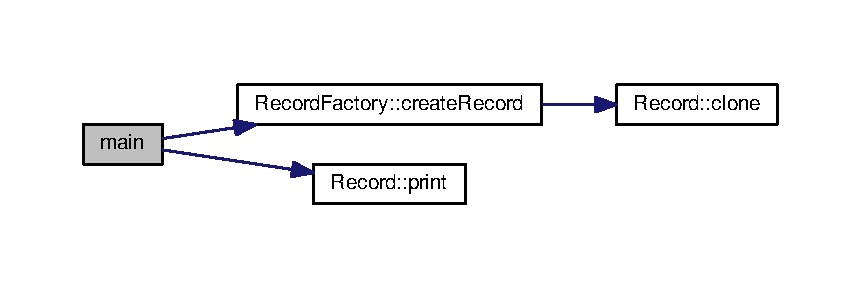
\includegraphics[width=350pt]{Prototype_8cpp_ae66f6b31b5ad750f1fe042a706a4e3d4_cgraph}
\end{center}
\end{figure}



%--- End generated contents ---

% Index
\backmatter
\newpage
\phantomsection
\clearemptydoublepage
\addcontentsline{toc}{chapter}{Index}
\printindex

\end{document}
